%% AISB03.tex
%%
%% Example of use of the AISB03 style.
%%
%% Created by Fred Labrosse.
%% Comments and bugs to ffl@aber.ac.uk
%%
%% Last modification: 22/11/2002
%%

\newif\ifnote
\ifx\notepaper\undefined
  \notefalse
\else
  \notetrue
\fi

\newcommand{\pflist}
  {	\renewcommand{\labelitemi}{$\triangleright$}
	\setlength{\itemsep}{0mm}
	\setlength{\parsep}{0mm}
	\setlength{\partopsep}{0mm}
	\setlength{\topsep}{0mm}
	\setlength{\parskip}{0mm}    }

%%\documentclass[a4paper,10pt,twocolumn]{article}
\documentclass[letter]{epirob}

%%\usepackage{AISB03}
\usepackage{graphicx}

\newcommand{\citep}{\cite}

\newcommand{\dgrs}{$^{\circ}$}

\newcommand{\percent}{\%}

\begin{document}

%%\title{Bootstrapping vision through shared activity}
%%\title{Learning from shared activity as a precursor to imitation}

%%\title{A Developmental Approach to Embodied Vision}

\title{The Whole World in Your Hand:\\
Active and Interactive Segmentation}

%% Three approaches to active segmentation

%%\title{From action to objects to actions on objects}

%%\title{From action to objects to actions on objects}

%%\title{Learning from shared activity}

%% Use \institute to create an institute use \inst to reference them.

\author{Artur Arsenio$^{*}$ \and Paul Fitzpatrick$^{*}$ \and Charles Kemp$^{*}$ \and Giorgio Metta$^{**}$}

\affiliation{$^{*}$MIT AI Lab \\
    Cambridge, Massachusetts, USA 
  \and
  $^{**}$Lira Lab, DIST, Uiversity of Genova \\
    Genova, Italy}

%% \title, \author and \abstract MUST be specified before \maketitle.

\maketitle


We describe YARP, Yet Another Robot Platform, an open-source project
that encapsulates lessons from our experience in building humanoid
robots.  The goal of YARP is to minimize the effort
devoted to infrastructure-level software development
 by facilitating code reuse, 
modularity and so maximize research-level development and collaboration. Humanoid robotics is a ``bleeding edge'' field of research, with constant flux in sensors, actuators, and 
processors.  Code reuse and maintenance is therefore a significant 
challenge. We describe the main problems we faced and the 
solutions we adopted. 
In short, the main features of YARP include support for inter-process
communication, image processing as well as a class hierarchy
to ease code reuse across different hardware platforms. YARP
is currently used and tested on Windows, Linux and QNX6 which are common 
operating systems used in robotics. 

%With YARP, we lay the ground-work for long-term
%software development. [need to review this]



\section{Introduction}

YARP is written by and for researchers in humanoid robotics, who find
themselves with a complicated pile of hardware to control with an
equally complicated pile of software.

%YARP includes modules to facilitate software development on
%humanoid robots, including abstractions for the operating system,
%image processing, physical devices, mathematical operations, etc.
%
At the time of writing, running decent visual, auditory, and tactile
perception while performing elaborate motor control in real-time
requires a lot of processor cycles. The only practical way to get
those cycles at the moment is to have a cluster of computers. Every
year what one machine can do grows, but so also do our demands~--
humanoid robots stretch the limits of current technology, and are
likely to do so for the foreseeable future.
Moreover, software is in general tight to the hardware on which it runs.
This limits modularity and code reuse which, in turn, complicates software 
development and mantainability. In the last few years we have been developing
a software platform to ease these tasks and improve the software quality on 
our robotic platforms. 
We want to reduce the effort devoted to programming to increase the 
time spent doing research. At the same time, we would like to have 
stable robotic platforms to work with.
Today YARP is a platform for long-term software 
development for applications that are real-time, computation-intensive, 
and involve interfacing with diverse and changing hardware. It is is 
successfully used on several platforms in our research Laboratories. 
The diversity of contexts on which it has been applied
show that our efforts have been somehow successful [reference table?].


\begin{table}
\centerline{\small
\begin{tabular}{|l|c|c|c|}
\hline
Robot&Laboratory&size&OS\\
\hline
Babybot&LIRA-Lab&13&Win/QNX6\\
Eurobot&LIRA-Lab&11&Win/QNX6\\
RobotCub&LIRA-Lab&3&Win\\
Obrero&MIT-CSAIL&4&Linux/OSX\\
Mertz&MIT-CSAIL&4&Linux\\
Domo&MIT-CSAIL&6&Linux\\
COG&MIT-AILab&30&QNX4/Linux\\
Kismet&MIT-AILab&12&Linux/Win/QNX4\\
\hline
\end{tabular}
}
\caption {
Robots using YARP.
}
\end{table}


\section{Motivation}

Let us now introduce the main features of YARP by describing the general lessons
we have learned and applied to YARP.
%
%
%Here are some general lessons we have learned, and apply to YARP.
%
%\begin{itemize} \pflist
%\item {\bf One processor is never enough.}

\textit{\textbf{One processor is never enough.}}
Designing a robot control system as a set of processes running on a
set of computers is a good way to work. It minimizes time spent wrestling with
code optimization, rewriting other people's code, and maximizes
time spent actually doing research.  The heart of YARP is a
communications mechanism to make writing and running such processes as
easy as possible. Even where mobility is required this is not a limiting
factor if teathers or wireless communication are practical.

%\item {\bf Modularity.} 
\textit{\textbf{Modularity.}}
Code is better maintainaed and reused if it is organized in small processes 
each one performing a simple task. In a cluster of computers some processes 
are bound to specific machines (usually when they require particular hardware 
device), but most of the times they can run on any of the available computers. 
With YARP it is easy to write processes that are location independent and 
that can run on different machines without code changes. This allows to move 
processes across the cluster at runtime to redistribute the computational 
load on the CPUs or to recover from a hardware failure. 
YARP does not contain any means of automatically allocating processes as in 
some approaches like GRID \cite{grid}. Our apporach is that of leaving this
task to the user to act sensibly and allocate the processes. The rationale is that: i)
special interface hardware is necessarily to be controlled by the appropriate piece of 
software, and ii) in an etherogeneous network of processors, faster processors might 
need to be allocated differently from slower processors. The final behavior is that of 
a sort of ``soft real-time'' parallel computation cluster without the more demanding
requirements of a real-time operating system.

\textit{\textbf{Minimal interference.}}
%Ports were designed with the two-fold goal of reducing the interactions at large between 
%the various components of the robot controller and, simultaneously, to allow efficient 
%communication between interacting parts of the system. The bottleneck in this approach
%would eventually be the available bandwidth on the network. 
As long as enough resources are available, the addition of new components 
should minimally interfere with existing processes. This is important, since often 
the actual performance of a robotic controller depends on the timing of various signals. 
While this is not strictly guaranteed by the YARP infrastructure, the problem is in 
practice alleviated computationally by allowing the inclusion of more processors to 
the network, and from the communication point of view by the buffer policy.
%isolating sub-components.

%\item {\bf Stopping hurts.}
\textit{\textbf{Stopping hurts.}}
It is a commonplace that human cycles are much, much more expensive
than machine cycles.  In robotics, it turns out that the human
cost of stopping and restarting a process can be very high.
For example, that process may interface with some
custom hardware which requires a physical reset.  
That reset many need to be carefully ordered with respect to when the
process is stopped and started.
%
There may be other dependent processes that need to be restarted in
turn, and other dependent hardware. 
%
%
%
These ordering constraints are time-consuming to satisfy.
%
YARP does its part to minimize dependencies between processes,
% so only true physically required dependencies remain.  
communication channels between processes can come and go. 
A process that is killed or dies
unexpectedly does not require processes to which it connects to be
restarted. This also simplify cooperation between people, as
it minimizes the need to synchronize development on different  
parts of the system.
%
%In complex systems, with dozens of processes and hundreds of connections, it might become
%unpractical to shut down and restart the whole system every time a module is even slightly 
%changed. YARP allowing the run-time connection of channels permits the disconnection of 
%only those parts of the system that need to be, for instance, rebuilt. 
%
%\item {\bf Humility helps.}

\textit{\textbf{Humility helps.}}
Over time, sofware for a sophisticated robot needs to 
aggregate code written by many different people in many
different contexts.  Doubtless that code will have
dependencies on various communication, image processing,
and other libraries. Very often the operating system on which
software is developed pose similar constraints. This is especially
true with code that relies heavily on the services offered by the 
operating system (such as communication, scheduling, synchronization primitives, 
and device driver interface).
%
Any component that tries to place itself ``in control'' and has strong
constraints on what dependencies are permissible will not be tolerated
for long.  It certainly cannot co-exist with another component
with the same assumption of ``dominance''. 
Although YARP offers support for communication, image processing,
interfacing to hardware etc., it is written with an {\em open world}
mindset.  We do not assume it will be the only library used, and
endeavor to be as friendly to other libraries as possible.
%
YARP allows interconnecting many modules seamlessly without subscribing
to any specific programming style, language interface, 
or demanding specifications as for instance in CORBA~\cite{vinoski97corba}
or DCOM~\cite{dcom}. Such systems, although far more powerful than YARP,
require a much tighter link between the general algorithmic code and the 
communication layer.
We have taken a more lightweight approach: YARP is a plain library linked
to uses-level code that can be used directly just by instantiating appropriate classes.
%
% and communication does not require any diversion
% of pre-existing threads. That is, YARP is a plain library linked to user-level
% code and as such migration to YARP can be easily carried out a posteriori. 
%
% Systems such as CORBA~\cite{vinoski97corba}, although far more powerful than YARP, require 
%
% adhering to well-defined interface specificiations (nothing bad as such) but consequently 
%
% a much tighter link between the general algorithmic code and the communication layer.
%
% is much 
% stricter. 
%
%
%
Finally, other programming languages can access YARP as well, provided they
have means of linking and calling C++ code. We have successfully used
YARP from within Matlab or L~\cite{brooks90behavior}.

%It is userful to reserve
%that role for the occasional poorly-designed hardware device that
%assumes it is the center of the universe.

%\end{itemize}

\noindent
%
%The OS library contains the communication facilities described in
%section \ref{sec:communication} and classes implementing
%synchronization routines (like mutexes and semaphores) and
%threads. 
%
\textit{\textbf{Exploit diversity.}}
%
Different operating systems offer different
features. Sometimes it is easier to write code to perform a given task
on a platform as opposed to another. This can happen for example if 
device drivers for a given board are provided only on a specific platform or
if an algorithm is available open source on another. We decided to reduce the
dependencies with the operating system. For this we
use ACE~\cite{ACEBook}, an open source library providing a framework for
concurrent programming across a very wide range of operating
systems. YARP inherits the portability of ACE and has indeed been used and
tested on Windows, Linux and QNX 6.



YARP's core communication model was the survivor from an early humanoid robot
controlled by a set of Motorola 68332 processors, an Apple Mac, and a loose network
of PCs running QNX, Linux, and Microsoft Windows.  Communication was a
hodge-podge of dual-port RAM, QNX message passing, CORBA, and raw
sockets.  At one point, three incompatible communication protocols
layered over QNX message passing were in use simultaneously.  This
variety was a consequence of organic growth, as developers added new
modules to the robot.  YARP began as one of the communication
protocols built on QNX message passing.  A key, defining, feature of
YARP was that it was {\em broad-minded}: it was
implemented in the form of a library which placed minimal constraints
on user code; communication resources did not need to be allocated at
any particular time or place in a program; reading messages could be
blocking, polling, or callback based, etc. This meant it could be
easily added without disturbing existing code, and communication could
be moved across to the new protocol piece by piece.

%The basic YARP module is an IPC infrastructure that supports communication across a
%network exploiting different protocols. 
%

%The mathematical library provides classes and functions to handle
%vectors and matrices, together with a few algebraic routines like
%single value decomposition, QR and LU factorization.

%More details about the image processing library and the device driver
%library can be found in the next sections.


%%
\section{Motivation}

We are highly motivated.




\section{Active Segmentation}

Gives a sketch of the min-cut algorithm and how it is applied to
this domain.

\begin{figure*}[tbh]
\begin{center}
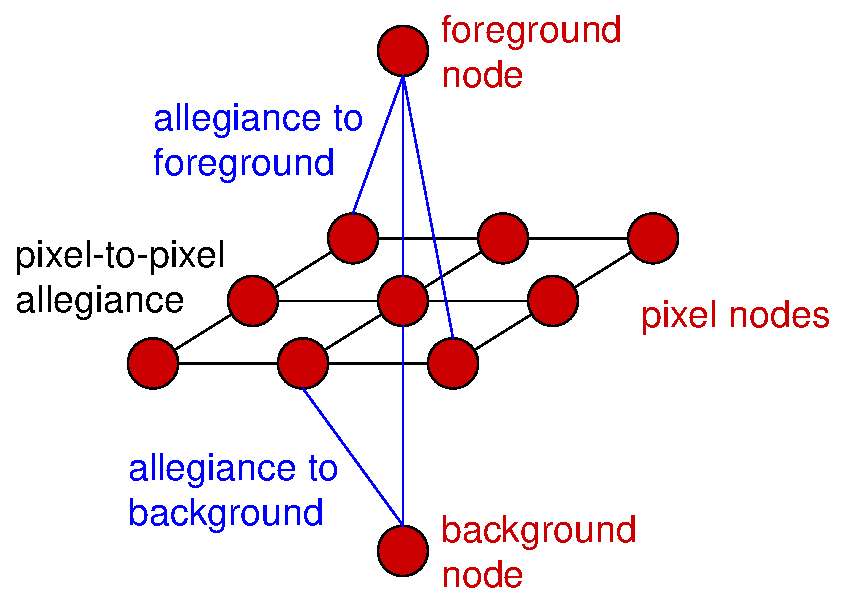
\includegraphics[width=7cm]{cut-graph1.eps}
\hspace{1cm}
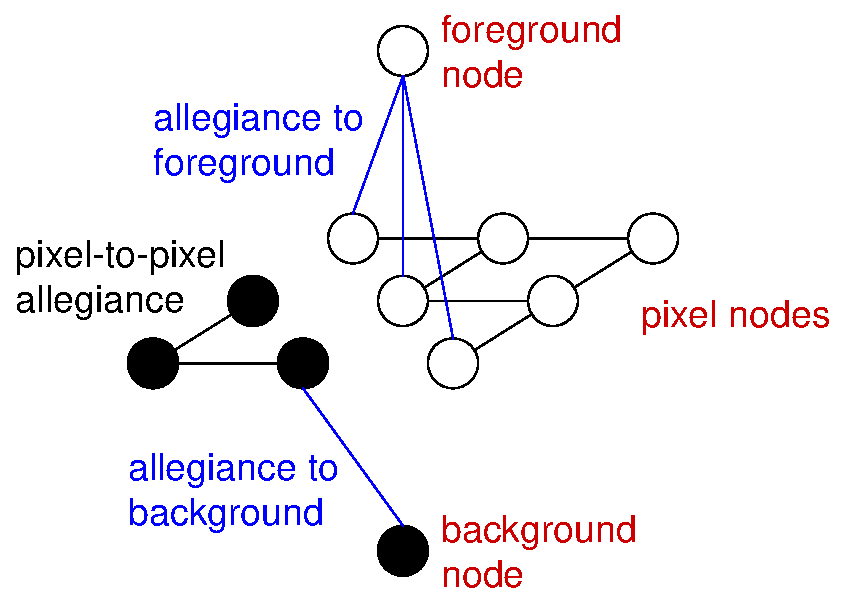
\includegraphics[width=7cm]{cut-graph2.eps}
\caption{ 
\label{fig:cut-graph}
%
A simple example of the graph cut algorithm in operation.  
The left graph represents the output of the point-of-contact 
processing.  Edges in the graphs are weighted by how much
it will cost to split connected nodes.  The bulk of the nodes
are in one-to-one correspondence with pixels in the image.
There are two extra nodes corresponding to the foreground and
background.  The goal is to split the graph into two by removing
edges.  The cost of the split is the sum of the weights on the 
edges removed.  There are good approximate algorithms for
finding a minimum cost solution [ref].
%
}
\end{center}
\end{figure*}

Use 16-connectivity (8 neighbors, plus cells connected by a
``knight'' move).

%
\begin{figure}[tb]
\begin{center}
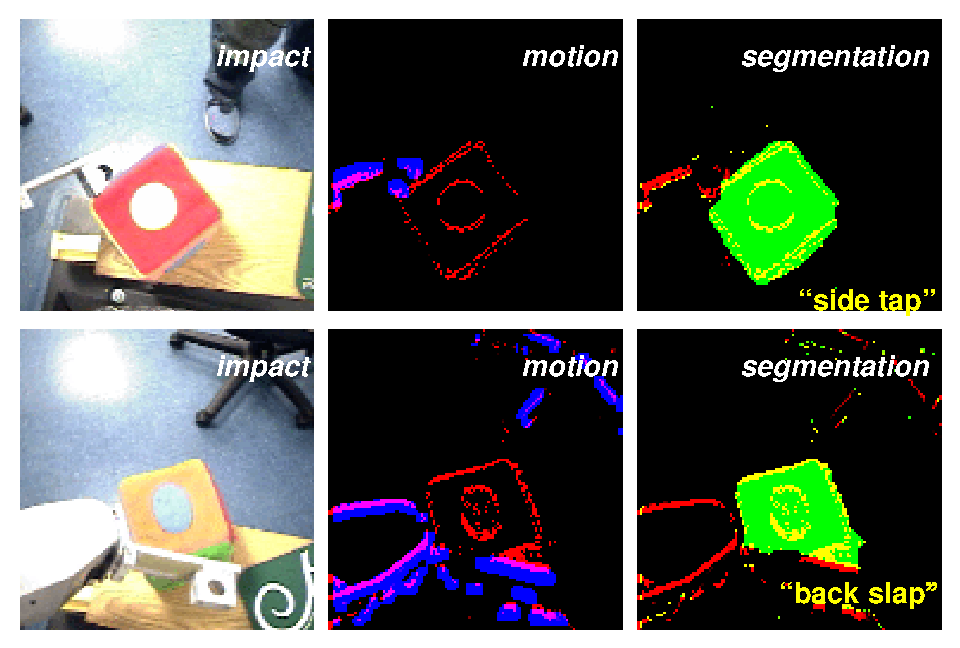
\includegraphics[width=\columnwidth]{segmentation-detail.eps}
\caption{ 
\label{fig:poking-segmentation}
%
Cog batting a cube around.  The top two rows show the flipper poking
the object repeatedly from the side, turning it slightly.  The third
row shows Cog batting an object away.  The images in the first column
are frames prior to a collision.  The second column shows the actual
impact.  The third column shows the motion signal at the point of
contact.  The bright regions in the images in the final column show
the segmentations produced for the object. 
%
}
\end{center}
\end{figure}
%

\begin{figure}[tbh]
  \centerline{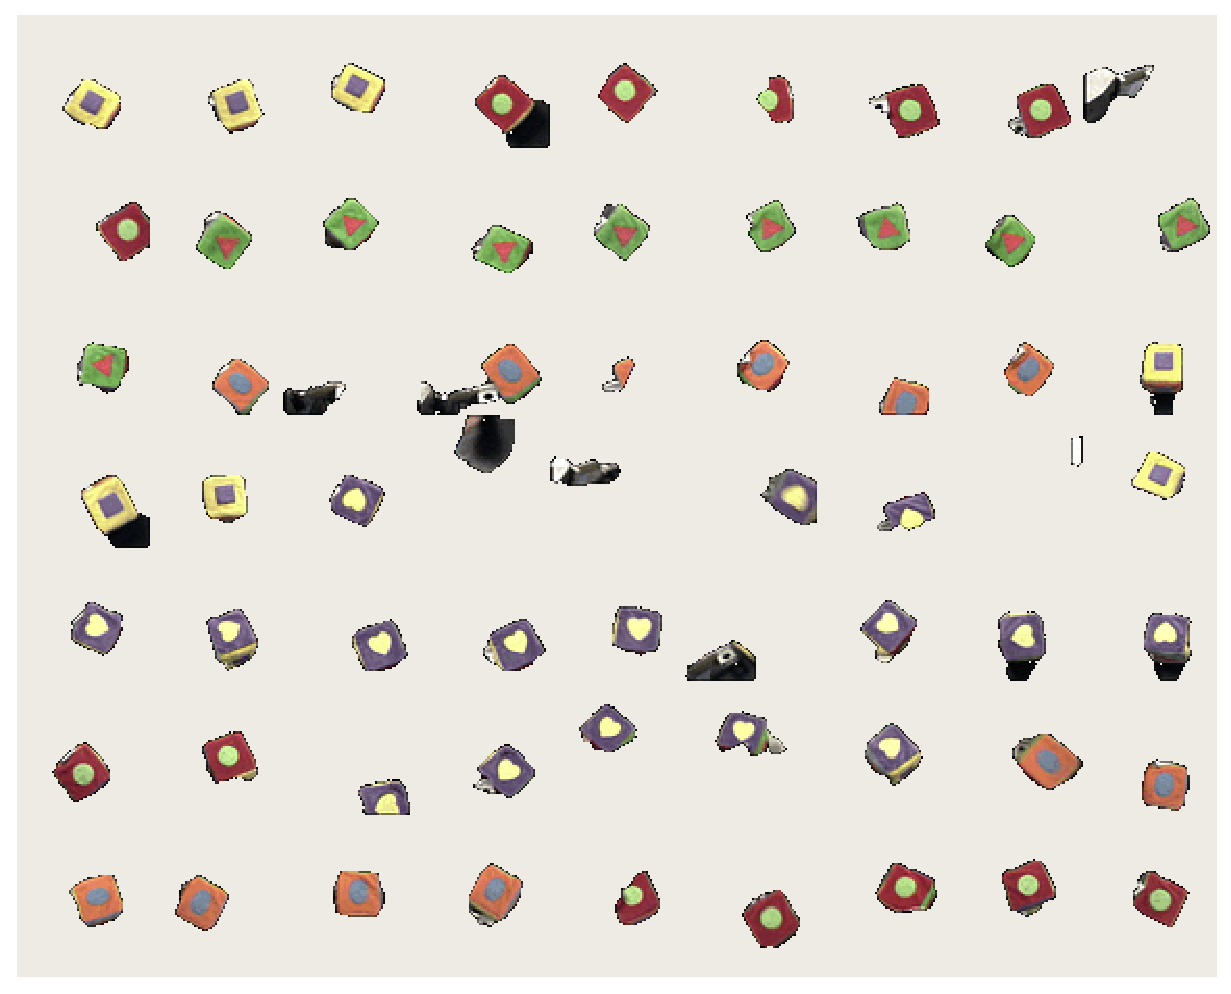
\includegraphics[width=2.5in]{experiment-montage}}
  \caption{Sample results}
  \label{fig:sample-results}
\end{figure}




%%\begin{figure}[tb]
\begin{center}
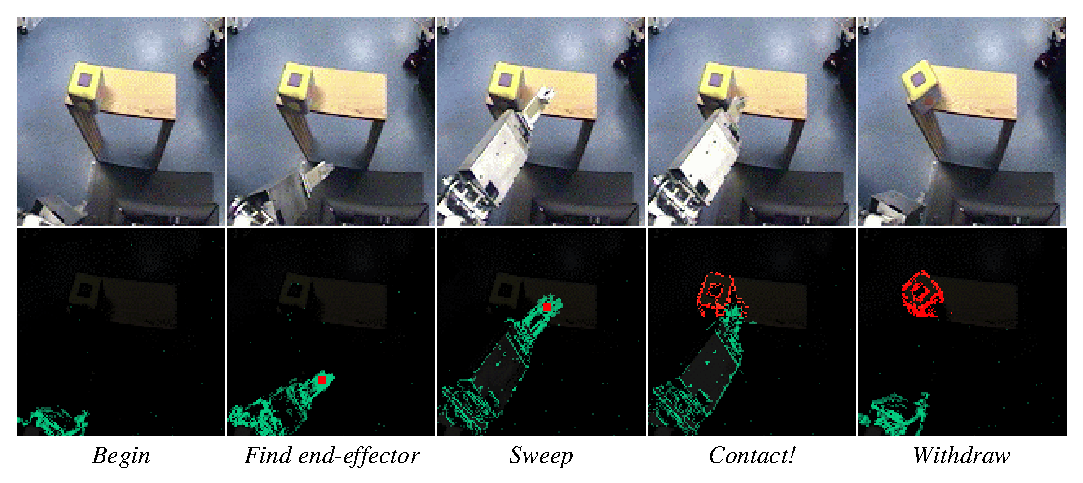
\includegraphics[width=\columnwidth]{poking-sequence.eps}

%%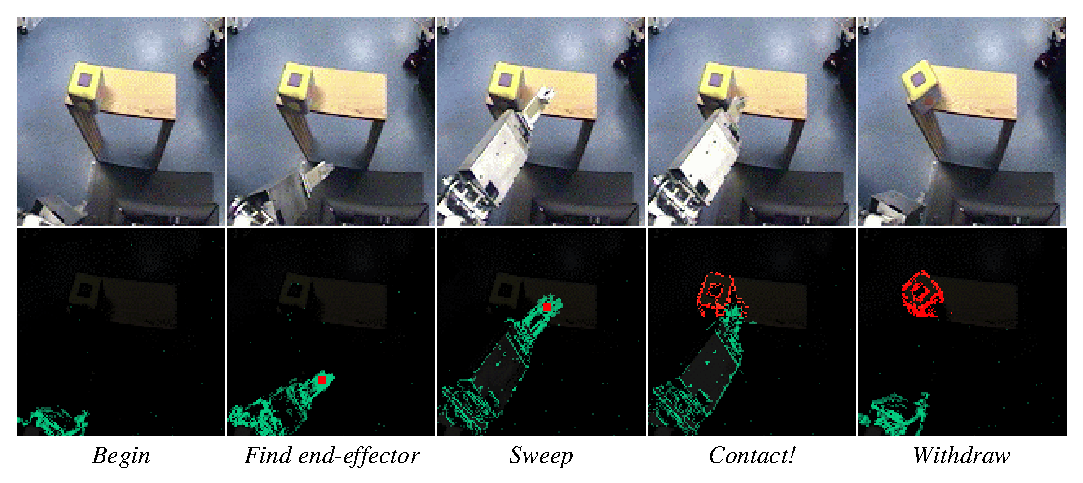
\includegraphics[width=\textwidth]{poking-sequence.eps}
%%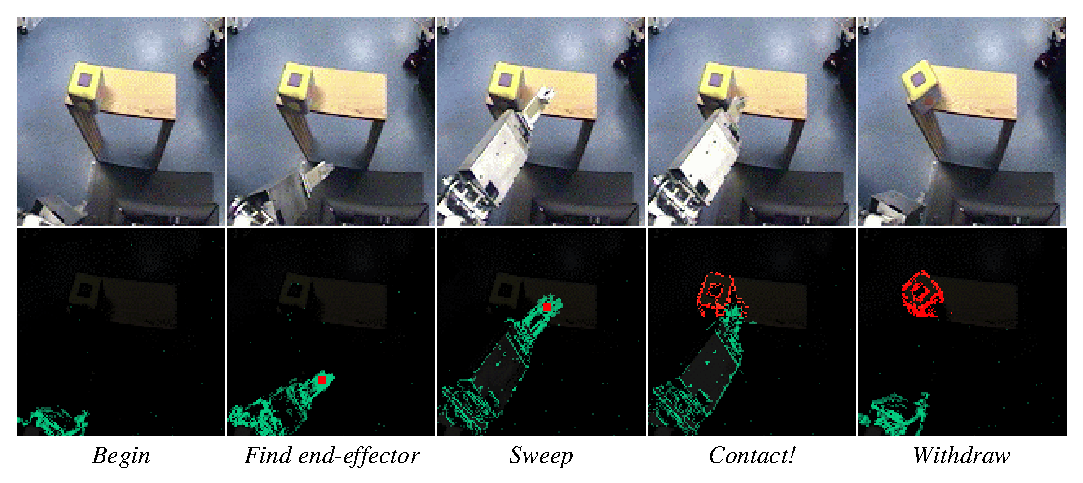
\includegraphics[width=14cm]{poking-sequence.eps}
\caption{ 
\label{fig:poking-sequence}
%
  The upper sequence shows an arm extending into a workspace, tapping
  an object, and retracting.  This is an exploratory mechanism for
  finding the boundaries of objects, and essentially requires the arm
  to collide with objects under normal operation, rather than as an
  occasional accident.  The lower sequence shows the shape
  identified from the tap using simple image differencing and flipper
  tracking.
%
}
\end{center}
\end{figure}



\section{Perceiving actions on objects}

Now that the robot knows something about its arm, it can start
to use it to explore its environment.
When the arm enters into contact with an object, one of several
outcomes are possible.  If the object is large, heavy, or otherwise
unyielding, motion of the arm may simply be resisted without any
visible effect.  Such objects are of little interest, except in their
role as obstacles, since the robot will not be able to manipulate
them.  But if the object is smaller, it is likely to move somewhat in
response to the nudge of the arm.  This movement will be temporally
correlated with the time of impact, and will be connected spatially to
the end-effector -- constraints that are not available in passive
scenarios~\cite{birchfield99depth}.  If the object is reasonably
rigid, and the movement has some component in parallel to the image
plane, the result is likely to be a flow field whose extent reflects
the physical boundaries of the object.  This visible response to
the robot's action can be used to refine its model of the object's
extent, which may be inaccurate.  For the example scene in
Figure~\ref{fig:setup-sequence} (a cube sitting on a table), the small
inner square on the cube's surface pattern might be selected as a
target.  The robot can certainly reach towards this target, but
grasping it would prove difficult without a correct estimate of the
object's physical extent.  In this section we show how the robot can
experimentally determine an object's extent using the same idea of
correlated motion used earlier to detect its own arm.

\subsubsection*{Making an impact}

Figure~\ref{fig:poking-sequence} shows how a ``poking'' movement can
be used to refine a target.  During this operation, the arm begins
by extending outwards from the resting position.  The end-effector (or
``flipper'') is localized as the arm sweeps rapidly outwards, using
the heuristic that it lies at the highest point of the region of optic
flow swept out by the arm in the image (the head orientation and
reaching trajectory are controlled so that this is true).  The arm is
driven outward into the neighborhood of the target which we wish to
define, stopping if an unexpected obstruction is reached.  If no
obstruction is met, the flipper makes a gentle sweep of the area
around the target.  This minimizes the opportunity for the motion of
the arm itself to cause confusion; the motion of the flipper is
bounded around the endpoint whose location we know from tracking
during the extension phase, and can be subtracted easily.  Flow not
connected to the end-effector can be ignored as a distractor.


The sequence shown in Figure~\ref{fig:poking-sequence} is about the
simplest case possible for segmenting the motion of the object, since most of the arm is stationary
when contact occurs.  In practice, we would rather have less
constraints on the motion of the arm, so we can approach the object
from any convenient direction.  We found that it was possible 
to attain this flexibility without losing the simplicity of object
segmentation that poking brings, by exploiting the unique
visual opportunity afforded by the moment of impact.


\ifverbose
For simplicity, the head is kept steady throughout the poking
operation, so that simple image differencing can be used to detect
motion at a higher resolution than optic flow.  Because a poking
operation currently always starts from the same location, the arm
is localized using a simple heuristic rather than the procedure described
in the previous section -- the first region of optic flow appearing
in the lower part of the robot's view when the reach begins
is assumed to be the arm.
\fi

\ifverbose
\begin{figure}[tbh]
\begin{center}
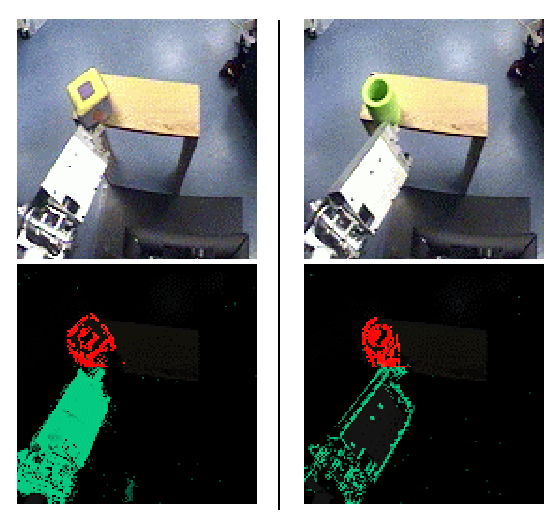
\includegraphics[width=\columnwidth]{cube-and-cylinder.eps}
\caption{ 
\label{fig:cube-and-cylinder}
%
  Poking can reveal a diffence in the shape of two objects without
  any prior knowledge of their appearance.
%
}
\end{center}
\end{figure}
\fi



\section{Detecting the point of collision}

Two components -- detecting the moment of impact, and extracting as 
much data as possible from the frames around it.

There are particular periods when the robot is attentive and fixating.
When this is so, it can detect visually when a collision occurs
between a moving object and a previously stationary object in view.
The principal task, then, is keep the motion of the moving object distinct
from that of the impacted object.

Brief introduction to image differencing and background subtraction.
Stationary camera assumption to facilitate pixel modeling.  Don't want
to keep head stationary, but can fixate for significant periods.

Image differencing is a very simple technique for detecting motion by
simply subtracting successive frames from a camera and looking for
pixel-level differences.  A moving object that has some contrast with
the background it is moving over will generate such differences.  Of
course, pixel differences can also be generated by changes in
illumination, cast shadows, computer monitors, movement of the camera
itself, etc.  A related technique called background modeling tries to
estimate the appearance of the fixed, stationary background of a 
scene, and then subtract the current view from the reference to 
detect new foreground.  While these techniques are not ideally
suited to a moving platform like our robot, they are short periods 
during which they can be useful.  In particular, when the robot is
fixating a target, we can do this.

Within the context of the robot fixating a target, we try to detect
the moment of impact precisely, so we can apply the (relatively) slow
segmentation optimization to a narrow interval of the video input and
maintain close to real-time performance.  A moving manipulator
colliding with an object will accelerate it, if it is not too massive.
If the object is rigid, the motion of the manipulator will be transmitted 
through it.  This transmission can be detected as a spreading motion
that is not plausibly generated by the manipulator itself.

Some assumptions that may fail: object not too heavy; object at least
semi-rigid; manipulator not moving above a certain speed; manipulator
not casting shadows on the object itself.  When the robot is poking the
object itself, it can control some of this.  If the object iself is
troublesome, then we potentially diagnose this, or just ignore it.

%%We are relying on some facts about optic flow.  When an object is ...

\begin{figure}[tbh]
  \begin{center}
    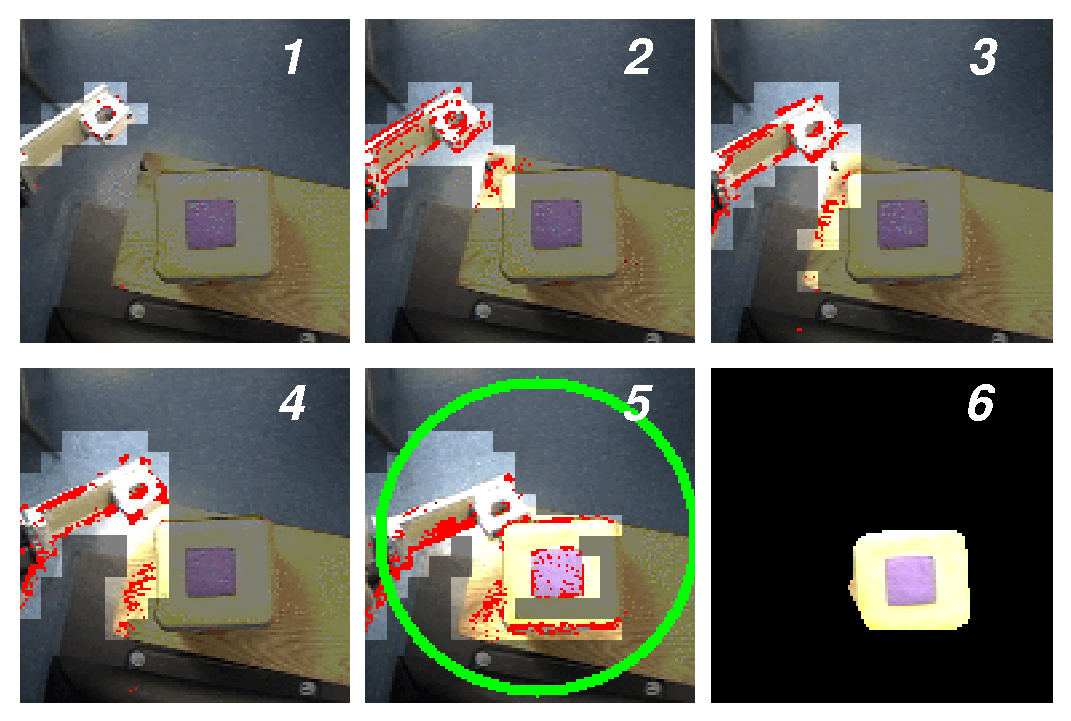
\includegraphics[width=12cm]{collision-detail}
  \end{center}
  \caption{
    The moment of impact is detected visually by the
    sudden expansion of motion away from the arm.  Motion before and
    after contact is compared to gather information for segmentation.
}
\end{figure}



\subsubsection*{An operational definition of objecthood}

The poking operation gives clear results for a rigid object that is
free to move.  What happens for non-rigid objects and objects that are
attached to other objects?  Here the results of poking are likely to
be more complicated to interpret -- but in a sense this is a good
sign, since it is in just such cases that the idea of an object
becomes less well-defined.  Poking has the potential to offer an
operational theory of ``objecthood'' that is more tractable than a
vision-only approach might give, and which cleaves better to the true
nature of physical assemblages.  The idea of a physical object is
rarely completely coherent, since it depends on where you draw its
boundary and that may well be task-dependent.  Poking allows us to
determine the boundary around a mass that moves together when
disturbed, which is exactly what we need to know for manipulation.  As
an operational definition of object, this has the attractive property
of breaking down into ambiguity in the right circumstances~-- such as
for large interconnected messes, floppy formless ones, liquids, and so
on.  Poking also gives the robot the opportunity
to collect many views of a single object, and so we can hope to deal
with recognizing objects like the cube shown in
Figure~\ref{fig:sample-results}, which look different from every side.


\begin{figure}[tbh]
  \centerline{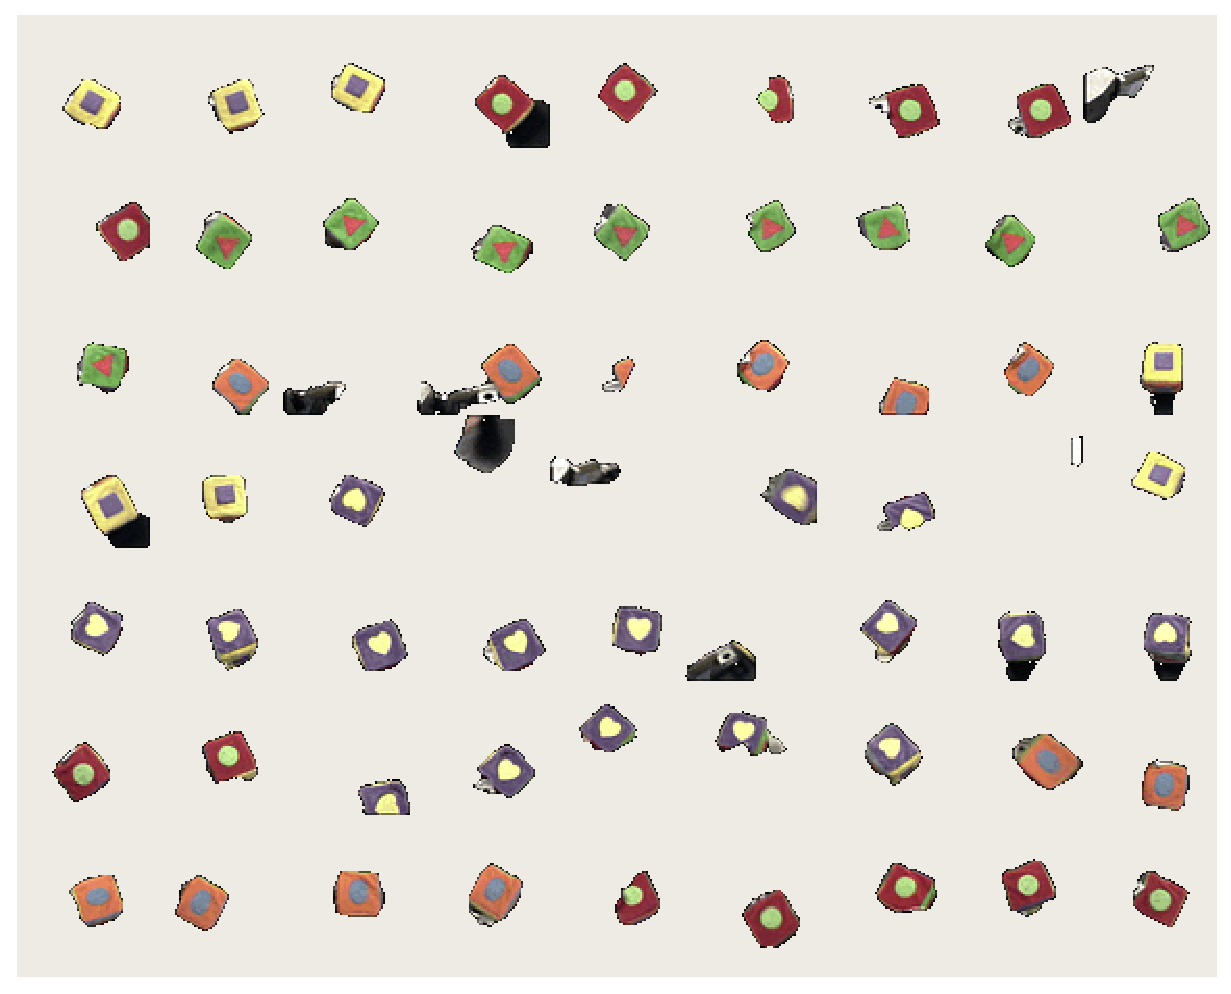
\includegraphics[width=9cm]{experiment-montage}}
  \caption{ 
  \label{fig:sample-results}
Results of a training session, where a toy cube was
  repeatedly offered to the robot for poking.  Each image of the cube
  corresponds to the segmentation found for it during a single poke.
  The most common failure mode is inclusion of the robot arm in the
  segmentation.  
}
\end{figure}



%%
\section{Learning about motion}


The robot tracks how an object moves after impact.
Pooling this data over all objects reveals how the movement of
the robot's arm correlates with the final movement of the object.

The robot was sensitive to color histogram, principal axis.
%
Some objects have preferred directions of motion.  For example,
a toy car tended to roll forward along its principal axis.
%
[Need a lot more here].
%
%%Figures~\ref{fig:observed-action} and \ref{fig:mimicked-action}.
Figure \ref{fig:mimicked-action}.


\ifnote
\begin{figure}[tb]
\begin{center}
%%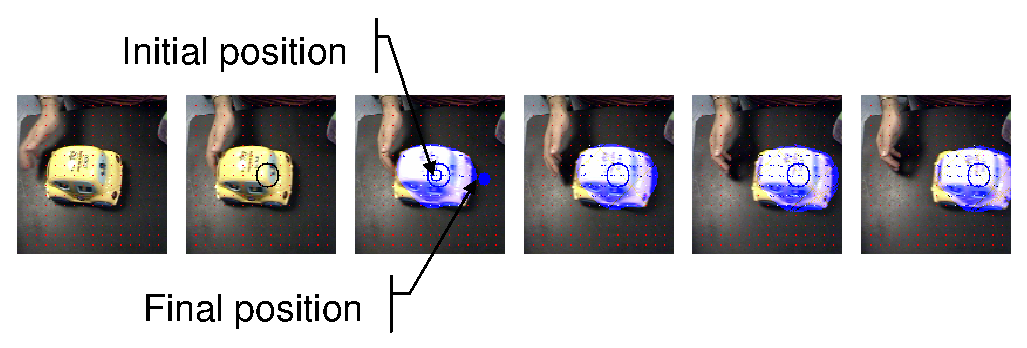
\includegraphics[width=\columnwidth]{observed-action.eps}
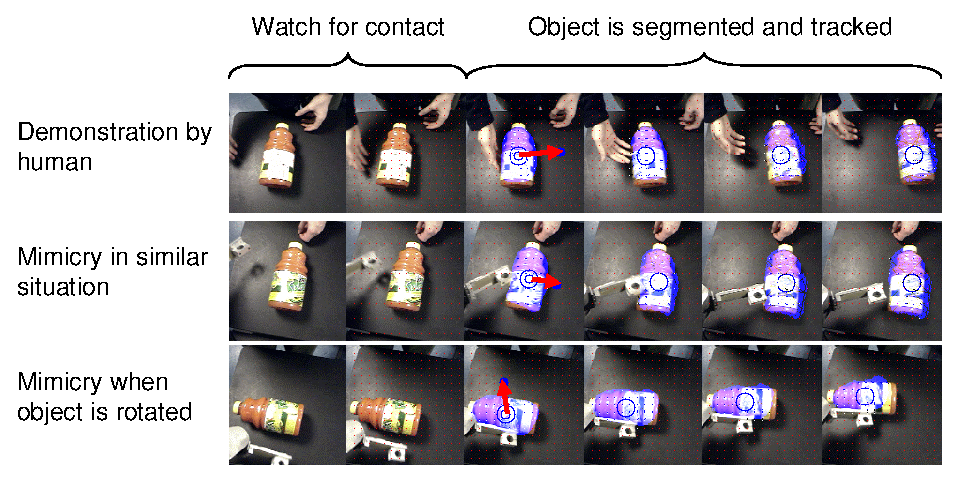
\includegraphics[width=\columnwidth]{fig-mimicry-bottle}
\caption{ 
\label{fig:observed-action}
%
Basic mimicry.  The first step in mimicking an action is to actually
be able to observe it.  The first sequence shows a human demonstration
of a poking operation.  Frames around the moment of contact are shown.
The object, after segmentation, is tracked for 12 frames using a
combination of template matching and optic flow.  The big circles
represent the tracked position of the bottle in successive frames.
The arrow displayed on the frame of contact ($3^{rd}$ from the left)
projects from the position at the time of contact and at the $12^{th}$
frame respectively.
%
In the second sequence, the bottle is presented to the robot in the
same orientation it had in the demonstrated action and the robot
repeats the observed action, a ``side tap''.  In the third sequence,
the car is presented at a different angle.  The appropriate action to
exploit the affordance and make the bottle roll is now a ``back
slap''.
%
%An example of observed sequence with tracking superimposed. 
%Frames around the
%moment of contact are shown. The object, after segmentation, is tracked for 12 
%frames using a combination of template matching and optic flow. The big circles
%represent the position of the toy car in successive frames. The two small circles
%(outline and solid) displayed on the frame of contact ($3^{rd}$ from the left) are 
%the position at the time of contact and at the $12^{th}$ frame respectively.
%
}
\end{center}
\end{figure}
\fi

\begin{figure}[tb]
\begin{center}
%%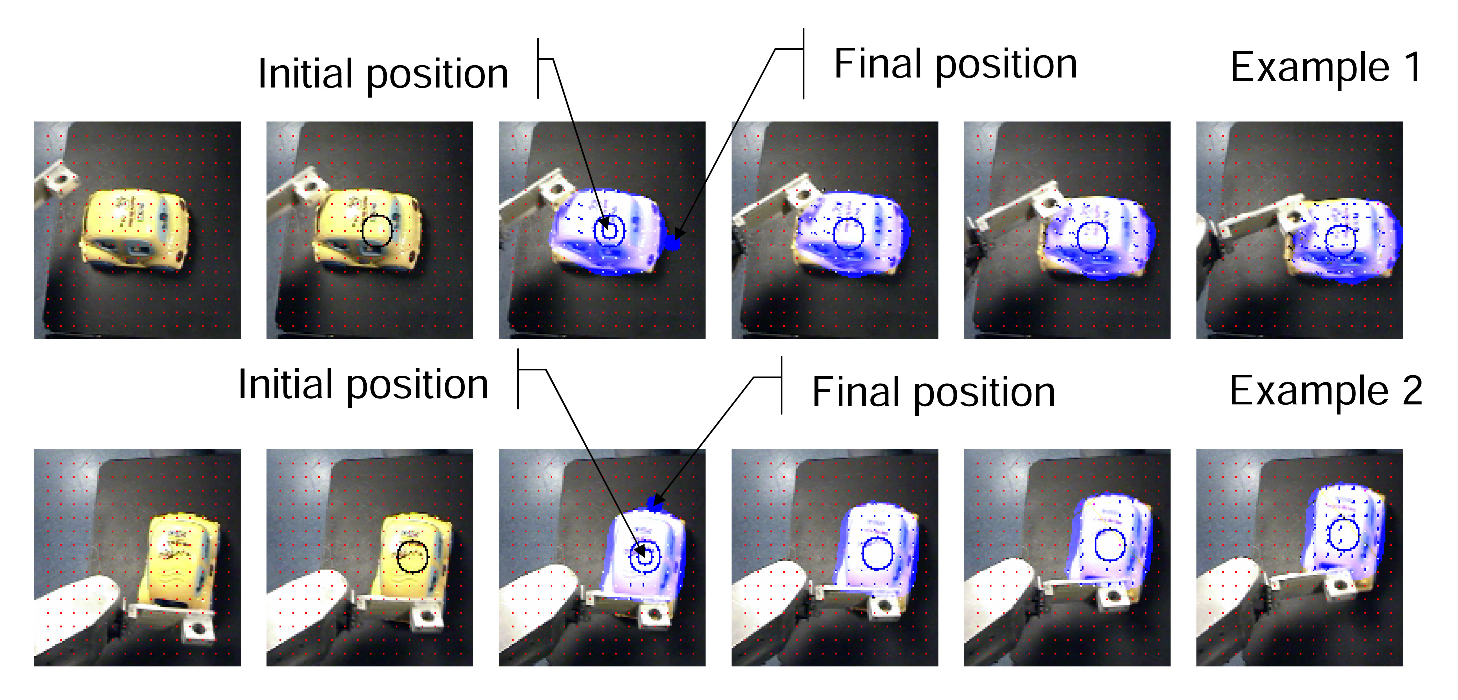
\includegraphics[width=\columnwidth]{mimicked-action.eps}
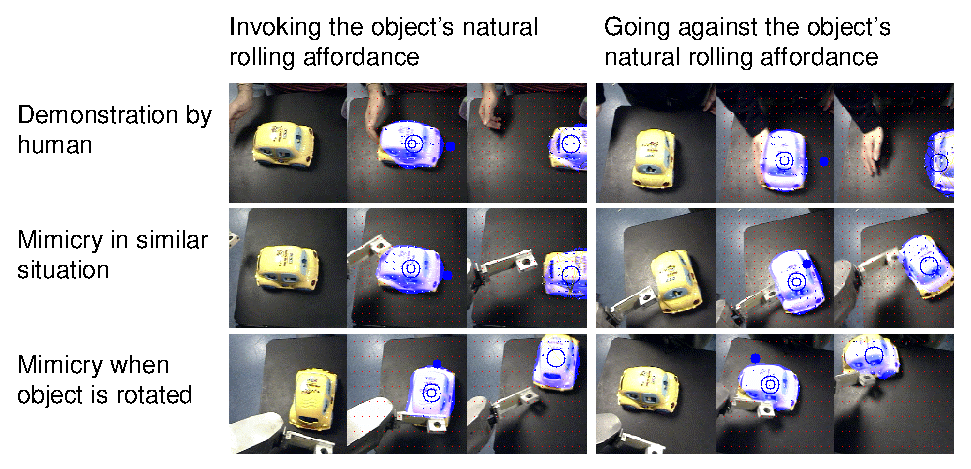
\includegraphics[width=\columnwidth]{fig-mimicry-awkward.eps}
\caption{ 
\label{fig:mimicked-action}
%
An extended mimicry example using the toy car.
The sequences on the left show the robot mimicking a human exploiting
the car's rolling affordance.  The sequences on the right show
what happens when the human hits the car in a contrary fashion, going
against its preferred direction of motion.  The robot mimics this 
``unnatural'' action, suppressing its usual behavior of trying to
evoke rolling.
%OUTDATED Two examples of mimicry following the observation in figure \ref{fig:observed-action} 
%where a human manipulator pokes the toy car exploiting the affordance (the car rolls). 
%In example 1 (top row), the toy car has the same orientation it had in the
%demonstrated action and the robot repeats the observed action. In example 2 (bottom), 
%the car is $90^\circ$ with respect to example 1. The appropriate action to exploit
%the affordance and make the car roll is thus a back slap. 
%
}
\end{center}
\end{figure}



%%

\section{Learning to recognize objects}

With any of the active segmentation behaviors introduced here, the
system can familiarize itself with the appearance of nearby objects.
This section is concerned with learning to locate and recognize those
objects whenever they are present, even when the special cues used for
active segmentation are not available.
%
The method described here has been applied to the poking method.

\subsection{Approaches to object recognition}

Physical objects vary greatly in shape and composition.  This variety
is reflected in their visual appearance.  Unfortunately, it is not a
straightforward matter to recover object properties from appearance,
since there are many other factors at work -- illumination, relative
pose, distance, occlusions, and so on.  The central challenge of
object recognition is to be sensitive to the identity of objects while
maintaining invariance in the face of other incidental properties.
%
There are at least two broad approaches to recognition, geometry-based
and appearance-based.

\subsubsection*{Geometry-based recognition}

Image formation is a geometric process, so one way to approach 
recognition is to model invariant geometric relationships that
hold for a particular class of object.  These relationships
can be between points, lines, surfaces or volumes.
%
They may be known for many possible views of the object, or just one.
When a new scene is presented, geometric relationships in it
are measured and matched against the model.
%
There are many details in what to measure and how to do the matching
(there is a good review in \cite{selinger01analysis}).
%
The main difficulty is the combinatorics of the search involved.
There are a lot of free parameters to search over when we try to
match an unsegmented scene to an object model -- in particular,
which elements in the scene correspond to the object, and 
what the transformation is between those elements and the object.
%
%One way to reduce this search is to use hashing.
For high-speed performance, geometric hashing is a useful technique
(for a review see \cite{wolfson97geometric}).  In this method,
geometric invariants (or quasi-invariants) are computed from points in
model (training) images, then stored in hash tables.  Recognition then
simply involves accessing and counting the contents of hash buckets.
%
One possibility for the geometric invariants is to take a set of
points selected by an interest operator, and use each pair of points
in turn to normalize the remainder by scale and rotation.  The
position of the normalized points can be stored in a 2D hash table, as
shown in Figure~\ref{fig:geometric-hashing}.  Invariants in 3D are
more difficult to achieve, but various solutions have been proposed.

\subsubsection*{Appearance-based recognition}

While the world is geometric in nature, geometric features are  not
particularly easy to extract reliable from images.  In
appearance-based recognition, the focus is shifted from the 
intrinsic nature of an object to properties that can be measured
in images of that object, including geometric properties but
also surface properties such as color or texture.
%
For example, \cite{swain91color} proposed using the set of colors
present in segmented views of an object as their representation.
Regions of an image that contain the same color mix (as determined
by histogram intersection) could contain the object.
%
Histogram back-projection can be used to quickly filter out regions
unlikely to contain the object, by assigning each pixel a weight based
on the frequency of its color in the histogram.  Some form of
region-growing method then accumulates this evidence to find plausibly
colored regions.  This method is very fast, and for objects with
distinctive colors it can be useful as a prefilter to more
computationally expensive processing.
%
%Histogram back-projection uses a very simple pixel-level feature
%(color) to locate objects.
Color is also intrinsically somewhat robust to scale and rotation,
but is sensitive to changes in the spectral profile of illumination.
%, which means that at detection time it is not
%necessary to search across these degrees of freedom (at least in the
%simplest implementation).

Many appearance-based methods are window-based.  A classifier is built
that operates on a rectangular region of interest within an image.
That window is moved across the entire image, at multiple scales, and
sometimes multiple orientations.  Responses of the classifier across
locations and scales are combined using various heuristics.  Variation
in orientation (rotation in depth) is typically dealt with by training
up multiple recognizers for various poses.  These poses can be sampled
quite sparsely, but still each pose requires iteration of the search
procedure.  Ther are ways to speed all this up, for example using a
cascade of classifiers that reject clearly non-target windows early,
devoting full analysis only to plausible targets.
%
The actual classifier itself can be based on eigenspace methods
or many other possibilities.

Probabilistic methods like Schiele.  Version with Roy.


\subsection{Hashing with rich features}

The approach used here is like geometric hashing, but uses
richer features that include non-geometric information.
%
Geometric hashing works because pairs of points are much more
informative than single points.  An ordered pair of points defines a
relative scale, translation, and orientation (in 2D).  Further points
may be needed for more general transformations, such as affine
or projective, or to move to 3D \cite[]{wolfson97geometric}.
%
But, even staying with the 2D case, using just two points is somewhat
problematic.  First of all, they are not at all distinctive -- any two
points in an image could match any two points in the model.  Hashing
doesn't require distinctiveness, but it would be a useful prefilter.
Secondly, there is no redundancy; any noise in the points will be
directly reflected in the transformation they imply.

One possibility would be to use triplets of points, or more.  Then we
have distinctiveness and some redundancy.  But we also have an
explosion in the number of possible combinations.  Pairs of points are
just about manageable, and even then it is better if they are drawn
from a constrained subset of the image.  For example, the work of
\cite{roy02learning} uses histograms of the distance and angles
between pairs of points on the boundary of an object for recognition.

In this work, pairs of edges (or more generally, any region with
well-defined and coherent orientation) are used instead of pairs of
points (Figure~\ref{fig:rich-hashing}).
%
Pairs of edges are more distinctive than pairs of points,
since they have relative orientation and size.  And if used carefully
during matching, they contain redundant information about the
transformation between image and model.  A disadvantage is that edges
are subject to occlusion, and edges/regions found automatically
many be incomplete or broken into segments.  But in all but the most
trivial objects, there are many pairs of edges, so this approach is
at least not doomed from the start.

The orientation filter developed earlier is applied to images, and a
simple region growing algorithm divides the image into sets of
contiguous pixels with coherent orientation.  For realtime operation,
adaptive thresholding on the minimum size of such regions is applied,
so that the number of regions is bounded, independent of scene
complexity.  In ``model'' (training) views, every pair of regions
belonging to the object is considered exhaustively, and entered into a
hash table, indexed by relative angle, relative position, and the
color at sample points between the regions (if inside the object
boundary).  

%Such features are very selective, yet quite robust to
%noise.

A useful extension of geometric hashing is coherency, where
each match implies a particular transformation, and only ``coherent''
matches are aggregated (for example, see \cite{lamiroy96rapid}).
%
This could be applied in the present instance.  For speed, an
abbreviated version is used here, where we filter by the centroid
location each match implies for the object (this is information we
would like to have anyway).  There is no coherence checking by scale
and orientation at the matching stage.  
%There are some advantages to
%this; principally that for objects with symmetries, we
%don't need to keep track of multiple possible transformations.
%
This procedure means that we perform object localization
simultaneously with matching.

Oriented regions are relatively sparse.  Experiments showed that on a
fast machine (800MHz) and at low resolution ($128\times 128$) it is
possible to use triplets of regions as features at close to real-time.
These can be very distinctive, and very redundant, and non-trivial
objects have very very many possible triplets.  But the frame-rate
was just too slow (approximately 1 Hz) to be worth using here.

At the other extreme, another possibility would be just to use single
edges.  But they are not very distinctive, and sampling colors at an
edge (generally a high-variance area) is problematic.


\section{Searching for a synthetic object in a synthetic scene}


\begin{figure}[tb]
\centerline{\includegraphics[width=\columnwidth]{fig-resegment-test5}}
\caption[Another example]{ 
%
%
A simple example of object localization: finding the circle in a
Mondrian.  
%
}
%%\label{fig:resegment-example2}
\end{figure}


As a simple example of how this all works,
consider the test case shown in Figure~\ref{fig:regment-mondrian}.
The system is presented with a model view of the
circle, and the test image.  For simplicity, the model view in 
this case is a centered view of the object by itself, so no
segmentation is required.  The processing on the model and
test image is the same -- first the orientation filter is applied, and
then regions of coherent orientation are detected.
For the circle, these regions will be small fragments around its
perimeter.  For the straight edges in the test image, these will
be long.  So finding the circle reduces to locating a region
where there are edge fragments at diverse angles to each other,
and with the distance between them generally large with respect
to their own size.  Even without using color, this is quite sufficient
for a good localization in this case.  The perimeter
of the circle can be estimated by looking at the edges that
contribute to the peak in match strength.
The algorithm works equally well on an image of many circles
with one square.


\subsection{Searching for real objects in synthetic scenes}

\begin{figure}[tb]
\centerline{\includegraphics[width=\columnwidth]{fig-resegment-test6}}
\caption[Searching for real objects in synthetic scenes]{ 
%
%
Looking for the best match to a cube found through poking in a
synthetic image of various approximations and distractors.
The superimposed red lines on the rightmost image
indicate the detected position of the object and the
edges implicated. 
The image on its immediate left shows the strength of
evidence for the object across the entire image, which lets us rank
the distractors in order of attractiveness. 
%
}
\label{fig:resegment-cube-yellow}
\end{figure}


In Figure~\ref{fig:resegment-cube-yellow}, we take a 
single instance of an object found through poking,
and search for it in a synthetic image containing an
abstract version of it along with various distractors.
The algorithm picks out the best match, and lets us
rand the distractors in order of salience.  It is clear that a yellow
square with anything in it is a good match, and having the internal
purple square adds another boost.  The closest distractor is a yellow 
square with a purple square inside it, rotated by 45\dgrs{}.




\begin{figure}[tb]
\centerline{\includegraphics[width=\columnwidth]{fig-resegment-example2}}
\caption[Another example]{ 
%
The cube being recognized, localized, and segmented in real images.
The image in the first column is one the system was trained on.
The image in the remain columns are test images.
Note the scale invariance demonstrated in the final image.
%
}
\label{fig:resegment-cube-real}
\end{figure}



\subsection{Recognizing real objects in real images}

Figure \ref{fig:resegment-cube-real}
shows examples of the cube being resegmented in real images.
%
%

Testing on a set of 400 images of four objects (about 100 each) being
poked by the robot, with half the images used for training, and half
for testing, gives a recognition error rate of about 2{\percent}, with
a median localization error of 4.2 pixels in a $128\times 128$ image
(as determined by comparing with the center of the segmented region
given from poking).  
%
By segmenting the image by grouping the regions
implicated in locating object, and filling in, a median of
83.5{\percent} of the object is recovered, and 14.5{\percent} of the
background is mistakenly included (again, determined by comparison
with the results of poking).
%





\section{Multiple objects simultaneously}

See Figure \ref{fig:resegment-multiple}.
Don't actually do this normally, deal with foveation
and egomap (described later).


\begin{figure}[tb]
\centerline{\includegraphics[width=\columnwidth]{fig-resegment-example}}
\caption[Hands-free segmentation]{ 
%
%Hands-free segmentation.
%The objects are on a very different table to the one 
%used during training.  
%Blue line indicates estimated
%boundary; white dot shows estimated location of object.
resegment multiple
%
}
\label{fig:resegment-multiple}
\end{figure}




\subsection{Online training}

Finally, Figure \ref{fig:resegment-online} shows recognition
and training occurring online.



\begin{figure}[tbh]
\centerline{\includegraphics[width=\columnwidth]{fig-online-recog2}}
\caption[Another example]{ 
%
This figure shows stills from a short interaction with Cog.
The area of the first frame highlighted with a square shows the state
of the robot -- the left box gives the view from the robot's camera,
the right shows an image it associates with the current view.
If the object confuses another object with what it has already seen,
such as the ball in the first frame, this is easily to fix
by poking.  IMPROVE THIS DESCRIPTION
%
}
\label{fig:resegment-online}
\end{figure}


\begin{figure}[tb]
\begin{center}
\includegraphics[width=\columnwidth]{fig-flipper-detect}
\caption{ 
\label{fig:flipper-detect}
%
This doesn't really need to be in the paper.
%
}
\end{center}
\end{figure}



%%
\section{Learning actor appearance}


In a sense, poking provides the robot with an operational definition
of what objects are
%% (``things that move when poked'') 
by giving it an
effective procedure for learning about them.  It is not perfect -- for
example, the robot is effectively blind to objects that are too small
or too large -- but for objects at an appropriate scale for
manipulation, it works well.
Once the robot is familiar with a set of such objects,
%Once the robot is familiar with a set of objects in its environment
%that are the right scale for it to manipulate, 
we can go further and provide an operational definition of a {\em
manipulator} as something that acts upon these objects.  We can create
an effective procedure for learning about manipulators by simply
giving the robot a predisposition to fixate familiar objects.  This
enables the same machinery developed for active segmentation to
operate when a foreign manipulator (such as the human hand) pokes the
fixated object.  Of course the robot can easily distinguish
segmentations of its own arm from that of others simply by checking
whether it was commanding its arm to move towards the target at the
time.  The manipulator can be segmented in a manner similar to 
that discussed in Section~\ref{sect:poking}.
%by hypothesizing that it moves
%towards the object at a constant velocity in the period immediately
%preceding the moment of contact.  
%Estimating the velocity from the
%gross apparent motion allows the segmentation problem to be expressed
%in the form introduced in Section~\ref{sect:min-cut}, 
%where the
%foreground is now taken to be regions moving at the desired velocity,
%and the background is everything else.
Figure~\ref{fig:auto-proto-flipper}
shows results for this procedure.  The results are based on
relatively little data, yet are already
sufficient to pick out good prototype views for the robot and human
manipulator.
A procedure like this could be used to autonomously
train a recognizer for the human hand, which could then
be included in further operational definitions, expanding
the robot's domain of grounded knowledge ever outwards.

\begin{figure}[tb]
\begin{center}
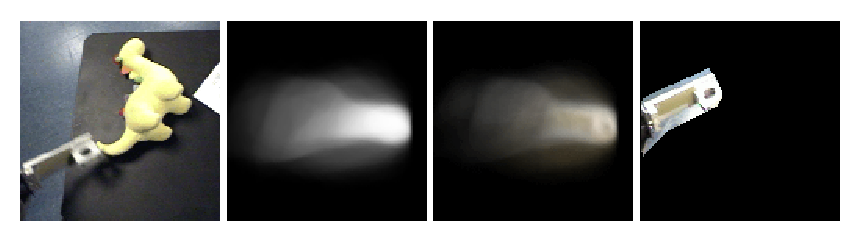
\includegraphics[width=\columnwidth]{fig-auto-proto-flipper.eps}\\
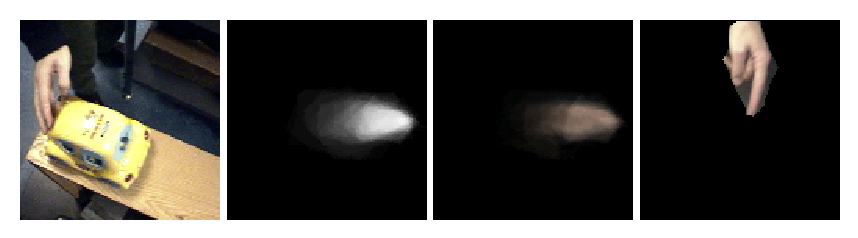
\includegraphics[width=\columnwidth]{fig-auto-proto-hand.eps}
\caption{ 
\label{fig:auto-proto-flipper}
%
The robot manipulator (top left) was automatically segmented during 20
poking sequences.  The segmentations were aligned and averaged, giving
the mask and appearance shown in the adjacent images.  The best
matching view is shown on the top right.  A similar result for the
human hand is shown on the bottom, based on much less data (5 poking
sequences, hands of two individuals).
%BREAK
%The human hand (see left) was automatically segmented during just 5
%poking sequences.  Hands of two different individuals were used.  The
%segmentations were aligned and averaged, giving the mask shown in the
%second image and the mean view shown in the third.  The best matching
%view is shown on the right.  
%Despite the paucity of the data,
%the mean view at least captures skin tone, which is sufficient to
%discard poor segmentations from consideration.
%
}
\end{center}
\end{figure}




%\section{Beyond segmentation}

%Making use of segmentation.




\begin{figure}[bt]
\centerline{
\includegraphics[width=8cm]{edge-samples-contrast}
}
\caption[The appearance of edges]{
%
The empirical appearance of edges.  Each $4\times 4$ grid represents
the possible appearance of an edge, quantized to just two luminance
levels.  The dark line centered in the grid is the average orientation
that patch was observed to have in the training data.
The upper set of patches are the most frequent ones that occur in
training data consisting of about 500 object segmentations.
The lower set of patches are a selection of patterns chosen to
illustrated the diversity of possible patterns that can occur.
The oriented features represented
include edges, thin lines, thick lines, zig-zags, corners
etc.  It is difficult to imagine a set of conventional
filters that could respond correctly to the full range of 
features seen here~-- all of which appeared multiple
times in object boundaries in real images.
%
}
\label{fig:seen-selected}
%%\label{fig:seen-selected-more}
\end{figure}


\ifnote
\begin{figure}[bt]
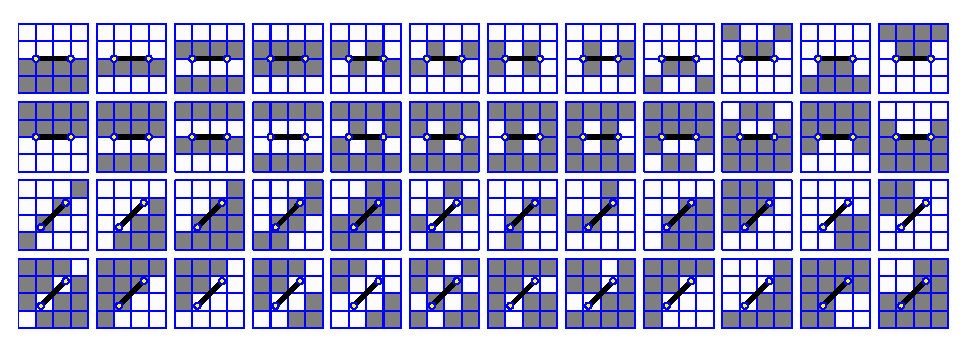
\includegraphics[width=\columnwidth]{seen-selected}
\caption
{
%
Edges have diverse appearances.  This figure shows 
the orientations assigned to a test suite
prepared by hand.  Each $4\times 4$ grid is a single test
edge patch, and the dark line centered in the grid is the orientation
that patch was observed to have in the training data.
The oriented features represented
include edges, thin lines, thick lines, zig-zags, corners
etc.  It is difficult to imagine a set of conventional
filters that could respond correctly to the full range of 
features seen here~-- all of which appeared multiple
times in object boundaries in real images.
%
}
\label{fig:seen-selected}
\end{figure}
\fi

\section{Building on segmentation}


As a specific example of development, the segmented views provided by
poking of objects and actors by poking can be collected and clustered
as shown in Figure~\ref{fig:clean-vision}.  Such views are precisely
what is needed to train up an object detection and recognition system,
and follow those objects and actors into other, non-poking contexts.

\begin{figure}[tb]
  \centerline{\includegraphics[width=10cm]{fig-poking-discovery}}
%%  \centerline{\includegraphics[width=\columnwidth]{fig-clean-vision}}
  \caption[How poking gets used]{
\label{fig:clean-vision}
%
The top row shows sample views of a toy car that the robot sees during
poking.  Many such views are collected and segmented as described
in~\protect\cite[]{fitzpatrick03first}.  The views are aligned to give an
average prototype for the car (and the robot arm and human hand that
acts upon it).  To give a sense of the quality of the data, the bottom
row shows the segmented views that are the best match with these
prototypes.  The car, the robot arm, and the hand belong to
fundamentally different categories.  The arm and hand cause movement
(are actors), the car suffers movement (is an object), and the arm
is under the robot's control (is part of the self).
%
}
\end{figure}

As well as giving information about the appearance of objects, the
segmented views of objects can be pooled to train up detectors for
more basic visual features~-- for example, edge orientation.  Once an
object boundary is known, the appearance of the edge between the
object and the background can be sampled along it, and labelled with
the orientation of the boundary in their neighborhood.
Figure~\ref{fig:seen-selected} shows an orientation filter trained up
from such data that can work at much finer scales than normally
possible when the filter is derived from an ideal edge model such as
that of \cite[]{chen00orientation}.  The ``catalog'' of edge appearances
found shows that the most frequent edge appearances is an ``ideal''
straight, noise-free edge, as might be expected (top of
Figure~\ref{fig:seen-selected})~-- but a remarkable diversity of other
forms also occur which are far less obvious (bottom of
Figure~\ref{fig:seen-selected}).

Can build on segmentation to learn about cool and useful stuff.

\subsection*{Learning about orientation}

A low-level example.

\subsection*{Learning to recognize objects}

A higher-level example.



\section{Learning about orientation}

Orientation is an important visual cue for many purposes, such as
object segmentation, recognition, and tracking.  It is associated with
neighborhoods rather than individual points in an image, and so is
inherently scale dependent.  At very fine scales, relatively few
pixels are available from which to judge orientation.
Lines and edges at such scales are extremely pixelated and
rough.
%
Orientation filters derived from analytic considerations, with
parameters chosen assuming smooth, ideal straight lines or edges (for
example, \cite{chen00orientation}) are more suited to larger
neighborhoods with more redundant information.
For fine scales, an empirical approach seems more promising, particularly
given that when the number of pixels involved is low, it is practical
to sample the space of all possible appearances of these pixels 
quite densely.

The data collected during segmentation allows us to explore how edges truly
look in ``natural'' images, by simply building up a catalog of edge
fragments seen around the boundaries of objects.  Of course, such a
catalog is only practical at small scales.  We worked with $4\times 4$
pixel windows, a size is chosen to be large enough to be interesting,
but small enough for the complete range of possible appearances to be
easily visualized.  Even at this scale, manual data collection and
labelling would be extremely tedious, so it is definitely advantageous
to have a robotic system to automatically compile and label a database
of the appearance of oriented features.
%
%, as shown in Figure~\ref{fig:separate-simple}.  
%Details of this procedure are given in
%Section~\ref{sect:experiment}.
These features were extracted by sampling image patches
along object boundaries, which were in turn determined 
using active segmentation.
The resulting catalog of edge appearances proved remarkably
diverse, although the most frequent appearances were indeed
the ``ideal'' straight, noise-free edge.

%Figures~\ref{fig:lines-all} and ~\ref{fig:seen-selected}.
%Figure~\ref{fig:seen-selected}.

\ifnote
\begin{figure}[tb]
\begin{center}
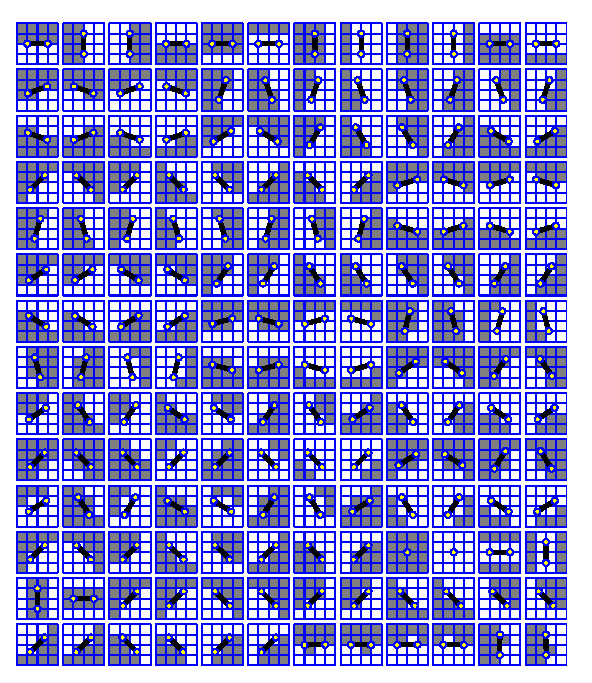
\includegraphics[width=\columnwidth]{seen-all}
\caption{
\label{fig:lines-all}
%
The most frequently observed edge appearances.  All patches
observed are replicated for all $90^{\circ}$ rotations, mirror flips,
and inversion of foreground/background.
%
The most frequent (top) are simple straight edges.
%
The line in the center of
each patch shows the orientation associated with that patch.  
%
After the straight edges, the completely empty patch
is common (produced in saturated regions), 
followed by a tube-like feature (third-last row)
where the boundary is visually distinct to either side of
the edge.
This is followed corner-like features and
many thousands of variations on the themes already seen.  
%
}
\end{center}
\end{figure}
\fi



+ Lorenzo's comments

-- I would stress the fact that modularity is a requirement and that processes need not to be aware of the machine on which they are running (the reason why we use names to identify the connections as opposed to static ip numbers).

-- We also keep GUI separate from the rest of the code

-- I tried to add something on OS independencies (and ACE, maybe we should say something more in the introduction or in the communication section) ?

+ Multiple people, shared resources, maximally independent projects.

+ We make it a rule that a process should never need to be restarted
  because of anything YARP does

+ Processes come and go.

+ Make streaming communication easy.

+ Name to ...




YARP client code is easy.

The package duration paradigm.

Giving control over buffer policy, but avoiding making user
think about it.

Gotchas:

+ pointers in structures

+ OnRead doesn't often get called.

+ sometimes expect both that all messages will get through, and
  that messages will get dropped for timeliness.

YARP

The principles of YARP:

+ Politeness.

+ Openness.

+ Playing well with others.

Motivations.

What type of robots we're dealing with.

History.

forgot to mention, important to AVOID UNNECESSARY COPIES


Adaptive scheduling?  Could be difficult to reason about.


The fundamental image class in YARP can easily become a {\em Proxy}
to image data stored externally or in an alternate representation.



\section{other projects}

IPC by Christopher Fedor and Reid Simmons, used in Carmen.
Check this: \cite{roy03IROS}



\section{Device Driver Example: YARPGenericFrameGrabber}

As an exemple we report here the structure of the generic frame grabber. The first layer is the YARPDeviceDriver which defines the methods open(), close() and IOCtl(). It also stores the function table that implements the interface of the drivere (m\_cmds); this table is allocated and initialized in the YARPDeviceDriver constructor. This table is correcly filled by the DERIVED class (see below).

{\small \begin{verbatim}
template <class DERIVED>
class YARPDeviceDriver
{
public:
	YARPDeviceDriver(int n_cmds);
	virtual ~YARPDeviceDriver();
protected:
	typedef int (DERIVED::*cmd_function_t)(void *);
	// function table
	cmd_function_t *m_cmds;

public:
	virtual int open(void *p) = 0;
	virtual int close() = 0;

	int IOCtl(int cmd, void *data)
	{
	  int ret = ((DERIVED *)
	            this->*m_cmds[cmd])(data);
	  return ret;
	}
};
\end{verbatim} }

In addition we defined the following messages:

{\small \begin{verbatim}
enum FrameGrabberCmd
{
  FCMDWaitNewFrame,
  FCMDAcquireBuffer,
  FCMDReleaseBuffer,
  FCMDGetSizeX,
  FCMDGetSizeY,
  FCMDSetContrast,
  ...
};
\end{verbatim} }

The first message waits for a new frame to be acquired. FCMDAcquireBuffer reserves the most recent frame and returns a pointer to it; the frame is released by the application by calling FCMDReleaseBuffer. The other messages are simple commands to set/get general parameters.

The YARPGenericGrabberAdapter is a virtual class which defines the interface for the adapter. In this case it is quite simple and consists only in the initialize() and uninitialize() methods. 

The last layer is a template class YARPGenericGrabber whose parameter is the adapter of a specific board. Part of the implementation of the YARPGenericGrabber is reported here:

{\small \begin{verbatim}
template <class ADAPTER>
class YARPGenericGrabber
{
protected:
	ADAPTER _adapter;
public:
	YARPGenericGrabber ();
	~YARPGenericGrabber ();

	int initialize (...)
	{
	  return  _adapter.initialize(...);
	}

	int uninitialize ()
	{
	  return _adapter.uninitialize();
	}

	int acquireBuffer (unsigned char **buffer)
	{
	  return _adapter.IOCtl(FCDMAcquireBuffer, 
	                        buffer);
	}

	int releaseBuffer (void)
	{
	  return _adapter.IOCtl(FCMDReleaseBuffer);
	}

	int setContrast(unsigned int contrast)
	{
	  return _adapter.IOCtl(FCMDSetContrast, 
	                        &contrast);
	}

	... //other methods
}
\end{verbatim} }

To instantiate and use the YARPGenericGrabber in our code we need to define the classes implementing the device driver and the adapter for the particular board we intend to use (respectively MyDeviceDriver and MyGrabberAdapter). MyDeviceDriver derives from YARPDeviceDriver. It implements open() and close() methods. The frame grabber interface is implemented in the form of a set of functions whose pointers are stored in m\_cmds. MyDeviceDriver does not need to implement all messages but only the subset of the ones that are meaningful for the board actually in use. This is perfectly safe because by default each entry of the table is initialized to point to an empty (but valid) function.

{\small \begin{verbatim}
class MyDeviceDriver : 
	public YARPDeviceDriver<MyDeviceDriver>
{
  MyDeviceDriver()
  {
    // fils function table
    m_cmds[FCMDAcquireBuffer] =
                     &MyDeviceDriver::acquireBuffer;
    m_cmds[FCMDReleaseBuffer] =
                     &MyDeviceDriver::releaseBuffer;
    m_cmds[FCMDFaitFrame] = 
                     &MyDeviceDriver::waitOnFrame;
    ...
  }

  // open and initialize the device
  int open(void *d);

  // close the device
  int close(void);

protected:
  // messages:
  int waitOnFrame(void *cmd);
  int acquireBuffer(void *buffer);
  int releaseBuffer(void *cmd);
  ...
}
\end{verbatim}}

 The MyGrabberAdapter implements only and all the methods defined in the YARPGenericGrabberAdapter. It also derives from MyGenericDeviceDriver to allow accessing the device driver from the higher level layer. A possible implementation is reported here:

{\small \begin{verbatim}
class MyGrabberAdapter: 
	public MyDeviceDriver,
	public YARPGenericGrabberAdapter
{
  int initialize(...)
  {
    MyDeviceDriver::open();
    MyDeviceDriver::IOCtl(FCMSetContrast, ...);
    ... // other initializations
    return YARP_OK;
  }

  int unitialize()
  {
    MyDeviceDriver::close();
    ...
  }
}
\end{verbatim}}

Having implemented the adapter and the device driver for our frame grabber, it is now sufficient to instantiate and use the YARPGenericGrabber as follows:

{\small
\begin{verbatim}

typedef YARPGenericGrabber<MyGrabberAdapter> 
                          YARPGrabber;

int main()
{
  YARPGrabber _grabber;
  // initialize device
  _grabber.initialize(..);
  
  bool done = false;

  while(!done)
  {
    // wait until a new frame is ready
    _grabber.waitOnNewFrame();
    // lock most recent frame and
    // get a pointer to it
    _grabber.acquireBuffer(&buffer);
    // ...
    // ...
    // release frame
    _grabber.releaseBuffer();
  }

  // close the device
  _grabber.uninitialize();
}
\end{verbatim}
}


\section{Zone of proximal development}

(this section is very vague)

For infants, the zone of proximal development is the
difference between what they can accomplish on their
own compared to what they can accompish with an
adult's support [CITE].

By loose analogy, we label a robot control system's ``zone of proximal
development'' to be the set of modules being actively added or worked
on by the programmer, against a background of pre-existing, operating
modules.  

YARP helps insulate existing modules from changes in this zone,
and leaves them in a good form for when the zone moves on.






\section{Discussion and Conclusions}

In this paper, we showed how causality can be probed at different
levels by the robot.  Initially the environment was the body of the
robot itself, then later a carefully circumscribed interaction with
the outside world.  This is reminiscent of Piaget's distinction
between primary and secondary circular
reactions~\cite{ginsburg78piaget}.  Objects are central to interacting
with the outside world.  We raised the issue of how an agent can
autonomously acquire a working definition of objects. 

In computer vision there is much to be gained by bringing a
manipulator into the equation.  Many variants and extensions to the
experimental ``poking'' strategy explored here are possible.  For
example, a robot might try to move an arm around {\em behind} the
object.  As the arm moves behind the object, it reveals its occluding
boundary.  This is a precursor to visually extracting shape
information while actually manipulating an object, which is more
complex since the object is also being moved and partially occluded by
the manipulator.  Another possible strategy that could be adopted as a
last resort for a confusing object might be to simply hit it firmly,
in the hopes of moving it some distance and potentially overcoming
local, accidental visual ambiguity.  Obviously this strategy cannot
always be used!  But there is plenty of room to be creative here.
%
%
\ifrev
%
There are also limitations in our current implementation that could
usefully be addressed.
%
The robot itself is not mobile, so its workspace is limited.  
%
There are also many constraints on the arm that make fine 
motor control impossible -- it cannot maintain all reachable 
poses indefinitely, and there is significant noise and some 
hysteresis in its analog sensors.
%
The robot will only attempt to reach towards a target that is 
actually accessible to its arm -- not too close, not too far, 
as determined using visual disparity.  In practice, this 
means that the ideal workspace is a table in front of the 
robot, and the motor control of the robot has been 
specifically tuned to work well in that situation.
%
A simple attention system and tracking mechanism are used to 
bring the robot's attention to a target.  This phase can fail 
if the robot gets distracted by some more salient (but 
unreachable) part of the scene.
%
Objects that move together are not individually segmented.
%
And segmentation does not always succeed, due to shadows,
or strong nearby edges.
%
\fi

The robotic experiments support the view that reaching, grasping, and recognition
can be learned by following a particular ontogenetic pathway without the
intervention of an external teacher.
This pathway is consistent with and inspired by what is
known of this process in biological systems (primates/mammals).
%although this evidence is rather sparse.
%
We have endeavored to build from as few innate components as possible, to
elucidate the visual and motor challenges faced by a learning robot rather
than simply solving them by fiat.
%
%There is relatively little evidence to work with, but it is at least clear that the 
%sequence of events leading to object manipulation/recognition cannot take
%an arbitrary form unless we assume that some/many of its components are innate.
Although newborns show amazing abilities \cite{spelke-2000} such as early imitation 
\cite{meltzoff-moore-1977}, face detection, etc, there is also evidence 
that the maturation of the brain is far from complete at birth and
complex perceptual abilities require a long time to emerge \cite{kovacs00human}.
%
We have given a simple existence proof that object segmentation,
recognition and localization can develop without any prior knowledge
of visual appearance.  We have also shown that, without any prior
knowledge of the human form, the robot can identify episodes when a
human is manipulating objects that are familiar to the robot purely by
the operational similarity of the human arm and its own manipulator in
this situation.  We believe such demonstrations are important both in
their own right, and in their elucidation of a concrete series of
steps that lead to a desired behavior.  This may serve a useful
reference point from which to investigate the biological solution to
the same problem -- although it can't provide the answers, it can at
least suggests useful questions.

%
%This is important, since segmentation and recognition as usually expressed 
%suffer from a chicken-and-egg problem, where views of an object must be
%segmented before its appearance can be learned...

%We cannot claim that this is the only possible view but it is certainly one worth
%investigating. Rephrasing Berkeley we can say:
%\begin{quote}
%...objects can only be known by
%\emph{action}. Vision is subject to illusions, 
%which arise from \emph{many different} problems...
%\end{quote}
%that AI guys know far too well

%Could relate some of this to the embodied intelligence ideas
%of Brooks... particularly the working hypothesis.



%%
\section{Extras}


\begin{figure}[tbh]
  \begin{center}
    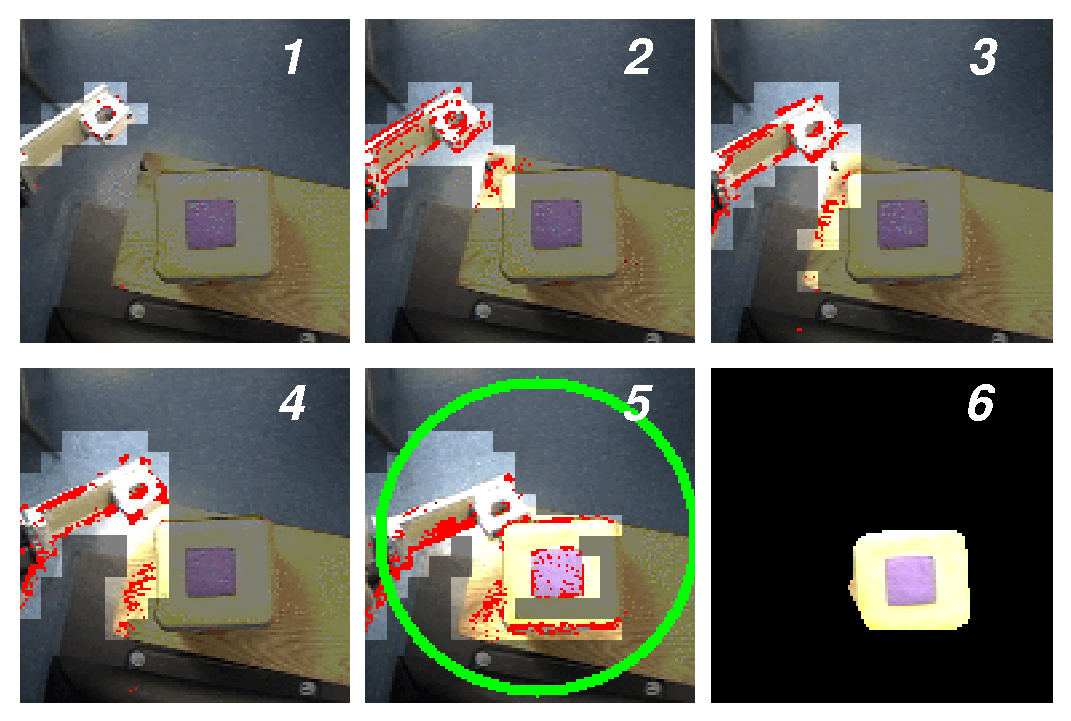
\includegraphics[width=2in]{collision-detail}
    \hspace{1in}
    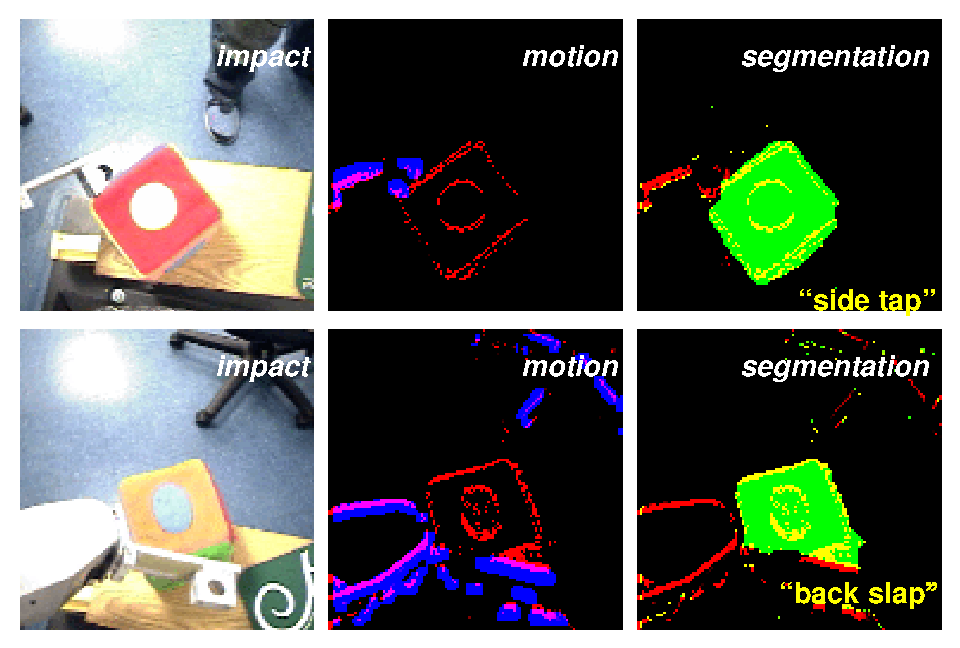
\includegraphics[width=2in]{segmentation-detail}
  \end{center}
  \caption{Part of the process}
\end{figure}

\begin{figure}[tbh]
  \centerline{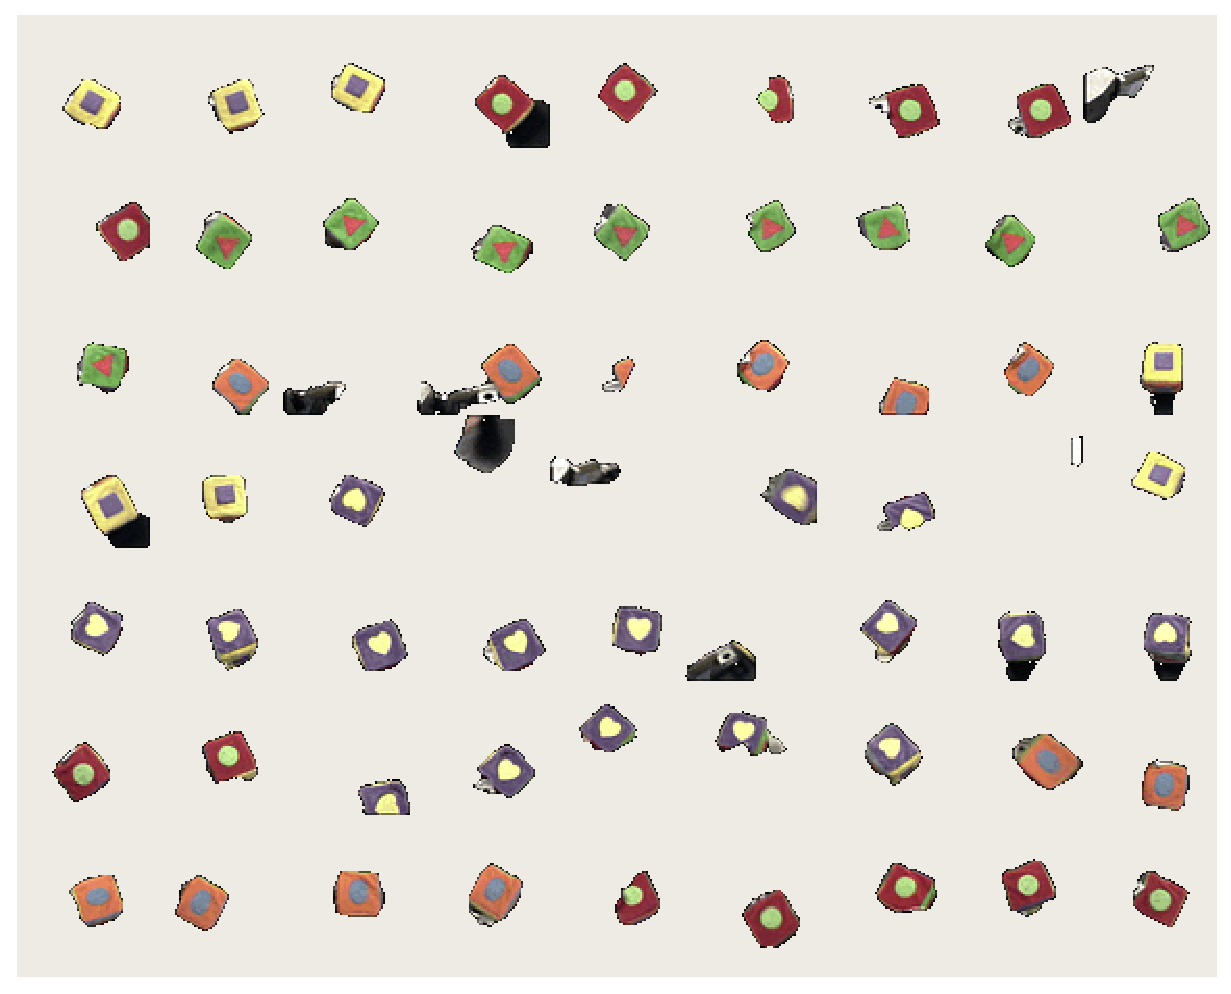
\includegraphics[width=2.5in]{experiment-montage}}
  \caption{Sample results}
  \label{fig:sample-results}
\end{figure}

\begin{figure}[tbh]
  \centerline{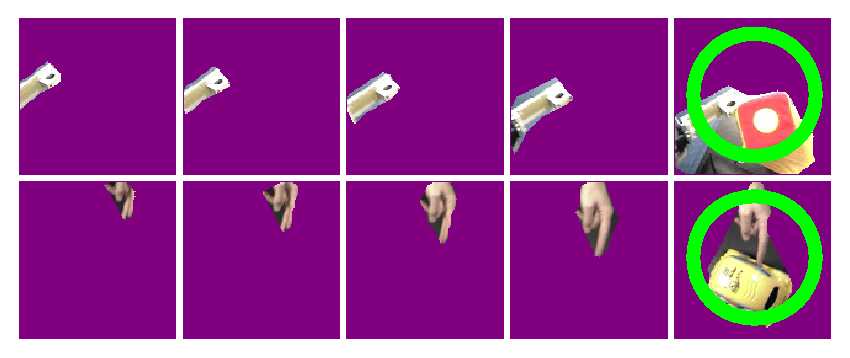
\includegraphics[width=2.5in]{manipulator-segment}}
  \caption{Segmenting the manipulator} 
  \label{fig:manipulator}
\end{figure}

\begin{figure}[tbh]
  \centerline{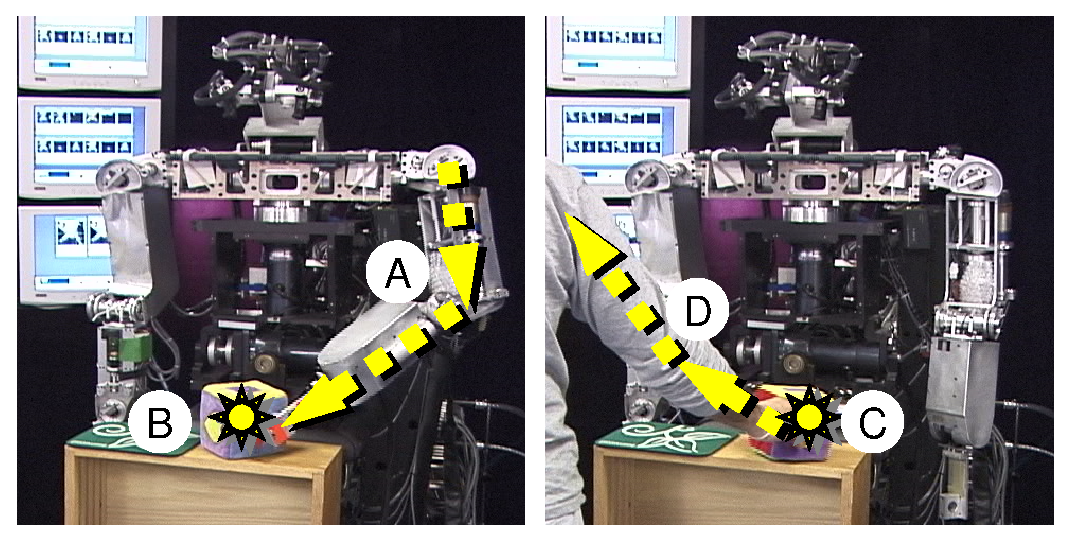
\includegraphics[width=2.5in]{tracing_causes}}
  \caption{foo} 
  %%\label{fig:foo}
\end{figure}


\begin{figure}[tbh]
  \centerline{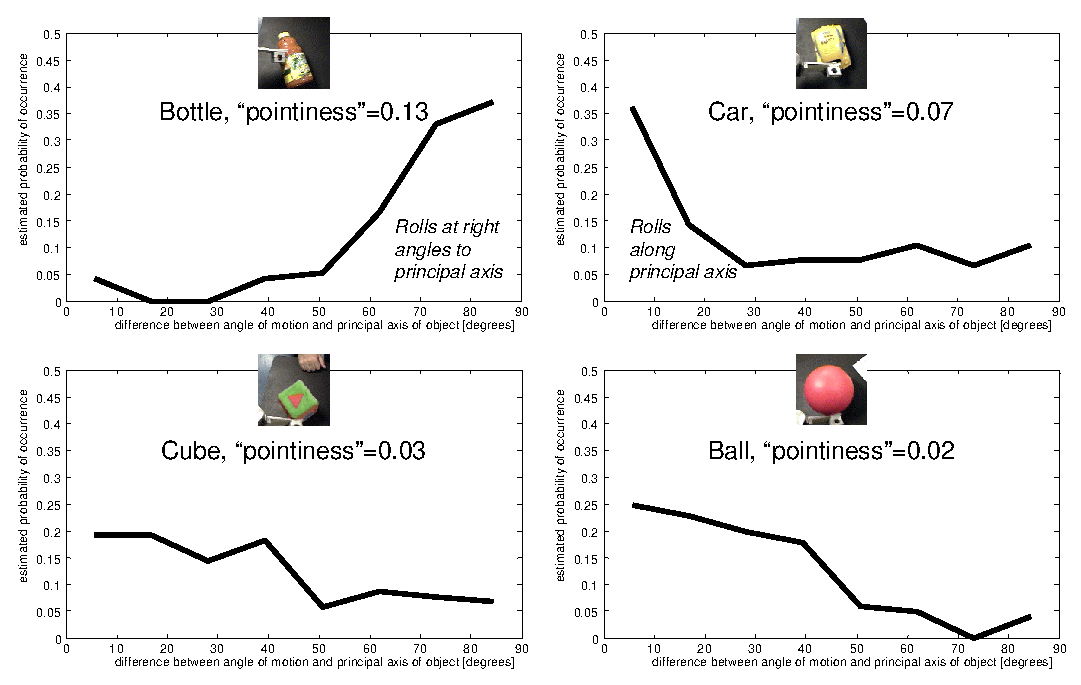
\includegraphics[width=2.5in]{rolling-graphs}}
  \caption{foo} 
  %%\label{fig:foo}
\end{figure}




\section*{Acknowledgments}
This work was supported by European Union grants RobotCub (IST-2004-004370)
and ADAPT (IST-2001-371173).



%%\bibliography{abbreviations,biblio}
% **** PUT YOUR OWN BIBLIOGRAPHY FILES IN HERE ****

\bibliographystyle{plain}

\bibliography{vision}


\end{document}

